\documentclass[../main.tex]{subfiles}

\begin{document}

\chapter{A New Approach for Processing Natural-Language Queries to Semantic Web Triplestores}
\begin{refsection}

This paper has been accepted to the WEBIST 2020 Springer journal.
We were invited to submit... %TODO

\label{chapter:webist2019journal}

%INTRODUCTION:
\section{Introduction}
\label{webist2019journal:intro}
This is an extended version of the paper by Frost and Peelar \cite{frostpeelar2019} that was presented at WEBIST 2019 in Vienna, Austria.  That paper was selected as one of the best papers at WEBIST 2019 and the authors were invited to submit an extended version for publication.  In this paper we expand upon the compositionality of our NLQI, including the parsing framework and semantic implementations, we introduce a novel method to accommodate superlatives using compositional semantics, and we discuss a novel approach to memoization and triplestore retrieval.  We also significantly expand upon how our NLQI is implemented.

\noindent We begin by describing a Natural Language Query Interface (NLQI) that we have built. We hope that the interface will motivate readers to look into our modifications to MS. In \Cref{webist2019journal:access}, we explain how our NLQI can be accessed through the Web. In \Cref{webist2019journal:compositionality}, we describe the compositional aspects of our NLQI.  In \Cref{webist2019journal:triplestore}, we describe the Semantic Web triplestore. In \Cref{webist2019journal:examples} we discuss example queries and their results, including examples of what are often referred to as ``non-compositional'' features of NL that our NLQI can handle. With each of the examples we provide an informal explanation of how the answer is, or could be, computed. In \Cref{webist2019journal:album}, we describe the new FDBR data structure which is central to our approach. In \Cref{webist2019journal:prep} and \Cref{webist2019journal:superlatives}, we describe how our system accommodates chained prepositional phrases with superlatives.  In \Cref{webist2019journal:relationaldb}, we describe how to use our approach with relational databases. In \Cref{webist2019journal:implementation}, we provide a system overview and implementation details on how our semantics are realized. \Cref{webist2019journal:relatedwork} discusses how our work fits into the framework of existing work in this area.  We close with \Cref{webist2019journal:futurework} and \Cref{webist2019journal:conclusions} where we discuss future research directions and our conclusions.

Much of our semantics is based on MS. We differ in these ways:

\begin{enumerate}
	\item We add events to the basic ontological concepts of entities and truth values.
	\item Each event has a number of roles associated with it. Each role has an entity as a value.
	\item For efficiency, we use sets of entities rather than characteristic functions of those sets as is the case in MS.
	\item We define transitive $n$-ary verbs in terms of sets of events, each with $n$ roles.
	\item We compute FDBRs, the novel data structure presented in this paper, from sets of events and use them in the denotations of transitive verbs and in computing results of queries containing prepositional phrases. Although not referred to as an FDBR, the use of relational images in denotations of verbs was first proposed by Frost and Launchbury in 1989 \cite{frost1989constructing}.
\end{enumerate}
We hope that this paper reawakens an interest in Compositional Semantics, in particular for NL query processing.

\section{How to Access our NLQI}
\label{webist2019journal:access}

Our NL interface is accessible via the following URL, and is speech enabled for both voice-in and voice-out in browsers that support the Web Speech API:

\begin{center}
	\url{http://speechweb2.cs.uwindsor.ca/solarman4/demo_sparql.html}
\end{center}

\section{Compositionality}
\label{webist2019journal:compositionality}

Compositionality is a useful property of any system as it facilitates understanding, construction, modification, extension, proof of properties,  and reuse in different situations. When building our system, we tried to make it as compositional as possible: a compositional syntax processor is systematically combined with a compositional semantics.

\subsection{The Compositionality of our Syntactic Processor}
\label{webist2019journal:compositionality-syntax}

Our parser is designed and built using the Haskell programming language, using parser combinators \cite{frost2008parser}. The approach enables parsers to be constructed as executable specifications of context-free grammars with explicit and implicit left-recursive productions, which is useful for defining grammars for NL. The result of applying our parser is the set of all parse trees for ambiguous grammars. The trees are represented efficiently using a Tomita-style \cite{tomita1985} compact graph in which trees share common components.

\noindent In 2008, Frost and Hafiz \cite{frosthafiz2008} demonstrated that it is possible to efficiently implement context-free parsing using combinators, with their approach having $O(n^4)$ complexity in the worst case and $O(n^3)$ complexity in the average case.

The following example was featured in Frost and Hafiz \cite{frosthafiz2008}. To demonstrate use of our combinators, consider the following ambiguous grammar from Tomita \cite{tomita1985}:
\begin{code}
	s    ::= np vp | s pp    np   ::= noun  | det noun | np pp
	pp   ::= prep np         vp   ::= verb np
	det  ::= "a"   | "the"   noun ::= "i"   | "man" | "park" | "bat"
	verb ::= "saw"           prep ::= "in"  | "with"
\end{code}
In this grammar, the non-terminal \texttt{s} stands for sentence, \texttt{np} for nounphrase, \texttt{vp} for verbphrase, \texttt{det} for determiner, \texttt{pp} for prepositional phrase, and \texttt{prep} for preposition.  It is left recursive in the rules for \texttt{s} and \texttt{np}.
The Haskell code below defines a parser for the above grammar using our combinators \texttt{term} (terminal), \texttt{<+>} (alternative), and \texttt{*>} (sequence) \cite{frost2008parser}:
\begin{code}
	data Label = S | ... | PREP
	s    = memoize S    $ np *> vp <+> s *> pp
	np   = memoize NP   $ noun <+> det *> noun <+> np *> pp
	pp   = memoize PP   $ prep *> np
	vp   = memoize VP   $ verb *> np
	det  = memoize DET  $ term "a" <+> term "the"
	noun = memoize NOUN
	$ term "i" <+> term "man" <+> term "park" <+> term "bat"
	verb = memoize VERB $ term "saw"
	prep = memoize PREP $ term "in" <+> term "with"
\end{code}
Parsers written in this fashion are highly compositional, and can be easily extended with new rules if needed.  Parsers constructed with our combinators have $O(n^3)$ worst case time complexity for non-left-recursive ambiguous  grammars (where $n$ is the  length of the input), and $O(n^4)$ for left recursive ambiguous grammars.  This compares well with $O(n^3)$ limits on standard algorithms for CFGs such as Earley-style parsers \cite{earley1970}.  The increase to $n^4$ is due to expansion  of  the  left  recursive non-terminals in the  grammar. The potentially exponential number of parse trees for highly-ambiguous input are represented in polynomial space as in Tomita’s algorithm.

\subsection{The Compositionality of our Semantics}

The semantics on which our system is based is similar to Montague Semantics. All phrases of the same syntactic category have meanings of the same semantic type. The meaning of all words and phrases are functions defined over sets of base terms which are entities, events and Boolean values. The meaning of a complex phrase is obtained by applying the functions which are the meanings of its parts, to each other in an order determined by the syntactic structure of the whole. Our system was easy to construct, and is easy to extend. Additional language features are accommodated by adding their syntactic structure and then defining their semantics by viewing the semantics of words and phrases of the same syntactic category.


\subsection{The Compositionality of the Whole NL Processor}

Our processor is built as an executable specification of a fully general attribute grammar. Compositional semantic rules are added to each syntactic production using the technique of Frost, Hafiz and Callaghan \cite{frost2008parser}. The attribute grammar is fully general as it can accommodate left recursive context-free grammars and fully-general dependencies between inherited and synthesized attributes. Haskell allows any computational dependency between attributes to be defined. Also, Haskell’s lazy evaluation strategy enables our language processor to be efficient. For example, no attribute computation is carried out until a successful parse has been obtained. We have also developed a variation of memoization using monads \cite{frost2008parser} in order to reduce the complexity of syntactic and semantic evaluation.
In the paper by Frost and Peelar \cite{frostpeelar2019} we discuss how we accommodate, using our compositional approach, various English phrases that are often given as examples of non-compositional constructs.

\section{The Triplestore that is Queried}
\label{webist2019journal:triplestore}
Our NLQI computes answers with respect to an \textit{event-based} Semantic Web triplestore containing data about the planets, the moons that orbit them, and the people who discovered those moons, and when, where and with what implement they were discovered.  Briefly, a triplestore is a database of 3-tuples, called triples, that have the form (\property{subject}, \textit{predicate}, \property{object}), where \property{subject}, \textit{predicate} and \property{object} are Uniform Resource Identifiers (URIs).

An \textit{event-based triple} has a \property{subject} that identifies an event rather than an entity \cite{peelar2016accommodating}. In these triples, the \textit{predicate} identifies a \textit{role} through which the \property{object} participates in the event.  That is, an event-based triple $(e,r,o)$ expresses that $o$ participates in $e$ through role $r$.
We call $o$ the event $e$'s ``$r$ \textit{property}''. For example, in \Cref{webist2019conf:evdiscover}, ``hall'' is event ``event1045'''s \property{subject} property. Triplestores consisting of event-based triples are called \textit{event-based triplestores}.

The advantage of event-based triplestores is that additional information about the events and entities participating in those events is immediately available. This is not the case in an entity-based triplestore, where some form of \textit{reification} is necessary to obtain additional information about a fact expressed in a triple.  For example, obtaining the location where ``\texttt{hall discovered phobos}'' in an entity-based triplestore, described by $(\hall, \discovered, \phobos)$, is not possible without reification.

We assume that each event will at minimum contain a role \textit{ev\_type} that identifies the type of the event, with the general expectation that events of the same type will contain similar roles.
This implies the existence of a schema that describes the types of roles that an event may contain.  As a consequence of this, each event could be equally well be represented by a row in a relational database.  We discuss this further in \Cref{webist2019journal:relationaldb}.

Going forward, when we refer to the type of an event or set of events, we are referring to their \textit{ev\_type} property.  Likewise, when we refer to events of a particular type, we are referring to events whose \textit{ev\_type} property corresponds to that type.  As a shorthand, we use $t$-type events to refer to events with type $t$.  For example, ``discover'' events refers to events that have \textit{ev\_type} property ``discover''.

The triplestore contains triples such as those in \Cref{webist2019conf:evdiscover} which represent the event in which \texttt{hall} (in the role of ``\property{subject}'') discovered \texttt{phobos} (in the role of ``\property{object}'') in 1877 (in the role of ``\property{year}'') with the \texttt{refractor\_telescope\_1} (in the role of ``\property{implement}'')  at the \texttt{us\_naval\_observatory} (in the role of ``\property{location}'').  Events representing set membership are represented as shown in \Cref{webist2019conf:evmember}.

%\begin{table}
%	\caption{Triples describing an event of type ``discover'' \cite{frostpeelar2019}. The full URIs of the events, roles, and entities have been omitted here.}
%	\label{webist2019journal:evdiscover}
%	\centering
%	\begin{tabular}{|l|l|l|}
%		\hline
%		Event & Role & Entity \\
%		\hline
%		event1045 &
%		subject &
%		hall \\
%
%		event1045 &
%		object &
%		phobos \\
%
%		event1045 &
%		ev\_type &
%		discover\_ev \\
%
%		event1045 &
%		year &
%		1877 \\
%
%		event1045 &
%		location &
%		us\_naval\_observatory \\
%
%		event1045 &
%		implement &
%		refractor\_telescope\_1 \\
%		\hline
%	\end{tabular}
%\end{table}
%\begin{table}
%	\caption{Triples describing an event of type ``membership'' \cite{frostpeelar2019}.}
%	\label{webist2019journal:evmember}
%	\centering
%	\begin{tabular}{|l|l|l|}
%		\hline
%		Event & Role & Entity \\
%		\hline
%		event1128 &
%		subject &
%		galileo \\
%
%		event1128 &
%		object &
%		person \\
%
%		event1128 &
%		ev\_type &
%		membership \\
%		\hline
%	\end{tabular}
%\end{table}
The complete triplestore, which contains tens of thousands of triples, is hosted on a remote server using the Virtuoso software \cite{virtuoso} and can be accessed by following the link at the beginning of \Cref{webist2019journal:access}.

\section{Example Queries}
\label{webist2019journal:examples}

Our NLQI can answer millions of queries with respect to the triplestore discussed above. The NLQI can accommodate queries containing common and proper nouns, adjectives, conjunction and disjunction, intransitive and transitive verbs, nested quantification, superlatives, chained prepositional phrases containing quantifiers, comparatives and polysemantic words. In the following sections, we provide an informal explanation of how the answer is computed.  If a query is syntactically ambiguous, the results from each possible interpretation of the query are separated with a semicolon.

\subsection{Queries Demonstrating the Range of NL Features that our NLQI can Accommodate}
\label{webist2019journal:nlexamples}

\examplequery{\indent phobos spins}{True}

\examplequery{phobos is a moon}{True}

\examplespacing

\noindent The function denoted by \texttt{phobos} checks to see if $\entityassoc{phobos}$ is a member of the $\spin$ set, and secondly if $\entityassoc{phobos}$ is a member of the $\moon$ set.

\examplespacing

\examplequery{a moon spins}{True}

\examplequery{every moon spins}{True}

\examplequery{an atmospheric moon exists}{True}

\examplespacing

\noindent The function denoted by ``\texttt{a}'' checks to see if the intersection of $\wordset{moon}$ and $\wordset{spin}$ is non-empty. The function denoted by ``\texttt{every}'' checks to see if $\wordset{moon}$ is a subset of $\wordset{spin}$. The denotations of \texttt{a} and \texttt{every} that we use are set-theoretic event-based versions of the denotations from MS which use characteristic functions.  The answer to the third query is obtained by checking if the intersection of $\wordset{atmospheric}$ and $\wordset{moon}$ is non-empty.

\examplespacing

\examplequery{hall discovered}{True}

\examplespacing

\noindent All of the events of type ``discover'' are collected together and are checked to see if $\entityassoc{hall}$ is found as the subject role value of any of them. If so, \textit{True} is returned.

\examplespacing

\examplequery{when did hall discover}{1877}

\examplespacing

\noindent The {\em year} property of the  events returned by ``\texttt{hall discover}'' (treated as ``\texttt{hall discovered}'') are returned.

\examplespacing

\examplequery{phobos was discovered}{True}

\examplespacing

\noindent All of the events of type ``discover'' are collected together and are checked to see if $\entityassoc{phobos}$ is found as the \property{object} role value of any of them. If so \textit{True} is returned.

\examplespacing

\examplequery{earth was discovered}{False}

\examplespacing

\noindent Earth was not discovered by anyone, according to our data.

\examplespacing

\examplequery{did hall discover phobos}{True}

\examplespacing

\noindent All of the events of type ``discover'' are collected together and are checked to create a pair $(s, \evs)$ for each value of the \property{subject} property found in the set of events. $\evs$ is the set of events to which the \property{subject} property is related through a discovery event.  Each pair is then examined to see if the function denoted by the object termphrase (in this case \texttt{phobos}) returns a non-empty set when applied to a set (called an \textit{FDBR}, which is described in \Cref{webist2019journal:album}) generated from the set of $\evs$ in the pair, and if so the subject of the pair is added to the set which is returned as the denotation of the verbphrase part of the query. The denotation of the termphrase at the beginning of the query is then applied to the denotation of the verbphrase to obtain the answer to the query. %(See \Cref{sec:album} for more detailed discussion of this process).

Owing to the fact that our semantics is compositional, the \property{subject} and \property{object} termphrases of the query above can be replaced by any termphrases, e.g.:

\examplespacing

\examplequery{a person or a team  discovered every moon that orbits mars}{True}

\examplequery{who discovered 2 moons that orbit mars}{hall}

\examplespacing

\noindent ``\texttt{who}'', ``\texttt{what}'', ``\texttt{where}'', ``\texttt{when}'' and ``\texttt{how}'' can be used in place of the \property{subject} termphrase. Different role values are returned depending on which ``\textit{wh}''-word is used in the query:

\examplespacing

\examplequery{where discovered by galileo}{padua}

\examplequery{when discovered by galileo}{1610}

\examplequery{every telescope was used to discover a moon}{True} (w.r.t.our data)

\examplequery{a moon was discovered by every telescope}{False}

\examplequery{a telescope was used by hall to discover two moons}{True}

\examplequerynl{which moons were discovered with two telescopes}{halimede laomedeia sao themisto}

\examplequery{who discovered deimos with a telescope that was used to discover every moon that orbits mars}{hall}

\examplequerynl{who discovered a moon with two telescopes}{nicholson science\_team\_18 science\_team\_2}

\examplequery{how was sao discovered}{blanco\_telescope canada-france-hawaii\_telescope}

\examplequery{how discovered in 1877}{refractor\_telescope\_1}

\examplequery{how many telescopes were used to discover sao}{2}

\examplequery{who discovered sao}{science\_team\_18}

\examplequerynl{how did science\_team\_18 discover sao}{blanco\_telescope canada-france-hawaii\_telescope}

\examplequery{which planet is orbited by every moon that was discovered by two people}{saturn; none} (ambiguous because ``\texttt{by two people}'' could apply to ``\texttt{discovered}'' or ``\texttt{orbited}'')

\examplequery{which person discovered a moon in 1877 with every telescope that was used to discover phobos}{hall; none} (ambiguous because ``\texttt{to discover phobos}'' could apply to ``\texttt{used}'' or ``\texttt{discovered}'')

\examplequery{who discovered in 1948 and 1949 with a telescope}{kuiper}

\subsection{Queries with ``Non-Compositional'' Structures}
\label{webist2019journal:noncompositional}

We agree that natural language has non-compositional features but believe that the non-compositionality is mostly problematic when the objective is to give a meaning to an arbitrary NL expression (i.e. an NL expression without a context). It is less problematic when answering NL queries. As illustrated below, the person posing the query, or the database or triplestore can provide contexts that help resolve much of the ambiguity resulting from non-compositional features. The advantages of a using a compositional semantics include:
\begin{enumerate}
	\item The answer to a query is as correct as the data from which it is derived,
	\item The meaning of sub phrases within a query can be discussed formally,
	\item The query language can be extended such that all existing phrases maintain their original meanings,
	\item The definition of syntax and semantics in the compositional semantics can be used as a blueprint for the implementation of the query processor.
\end{enumerate}
Some researchers have provided examples of what they claim to be non-com-\allowbreak positional structures in NL. For example, Hirst \cite{hirst1992semantic} gives the example of the verb ``depart'' which he states is not compositional because its meaning changes with the prepositional phrase(s) which follow it, and that the definition of compositionality needs to be modified to include the requirement that the function used to compose the meaning of parts must be systematic. We claim that our semantics for verbs is systematic as the denotations of subject and object termphrases, and the possibly empty list of prepositional phrases following the verb, are treated equally and are all used in the same way to filter the set of events of the type associated with the verb, before that set is returned as the denotation of the verb phrase. This is illustrated in the following queries:

\examplespacing

\examplequery{who discovered}{bernard bond cassini cassini\_imaging\_science\_team christy dollfus galileo etc...}

\examplespacing

\noindent No \property{subject}, \property{object} or prepositional phrase is given in the query, and so all events of type ``discover'' are returned by the verbphrase and the denotation of the word \texttt{who} picks out the \textit{subjects} from those events.

\examplespacing

\examplequery{where discovered io}{padua}

\examplespacing

\noindent No \property{subject}, or prepositional phrase is given in the query, and so all events of type ``discover'' are considered and filtered by the denotation of the \property{object} termphrase \texttt{io} and then, those that pass the filter are returned by the verbphrase and the word \texttt{where} picks out the location from those events. %(See section $\Cref{sec:examples}$ for more details).

\examplespacing

\examplequery{who discovered in 1610}{galileo}

\examplespacing

\noindent No \property{subject} or \property{object} is in the query so all events of type ``discover'' are considered and only those with the \property{year} property equal to 1610 pass the filter and then the denotation of the word \texttt{who} selects the subject which is returned.

\examplespacing

\examplequery{who discovered every moon that orbits mars with one telescope or a moon that orbits jupiter with a telescope}{one. ; none. ; none. ; bernard galileo kowal melotte nicholson perrine science\_team\_1 science\_team\_2 ; hall ; hall ; none.}

\examplespacing

\noindent As shown above, in our semantics, the \property{subject} and \property{object} termphrases are treated as filters, as are all prepositional phrases. Note that several results are returned here because the query is syntactically ambiguous.  We discuss solutions on how to best present the results of ambiguous queries to the user in \Cref{webist2019journal:ambiguity}.

\examplespacing

\examplequery{where discovered in 1610}{padua}

\examplequery{how discovered in padua}{galilean\_telescope\_1}

\noindent These queries retrieve the \property{location} and \property{implement} properties of the events of ``\texttt{discovered in 1610}'' and ``\texttt{discovered in padua}'' respectively.

\subsection{Extensions to the Semantics}
\label{webist2019journal:extend}

Some phrases containing nested quantifiers are given by some researchers as examples of non-compositionality. For example: ``a US diplomat was sent to every capital'' is often read as having two meanings which can only be disambiguated by additional knowledge. We argue that the person posing a query can express the query unambiguously if they are familiar with quantifier scoping conventions used by our processor, as illustrated in the following:

\examplespacing

\examplequery{christy or science\_team\_19 or science\_team\_20 or science\_team\_21 discovered every moon that orbits pluto}{False}

\examplespacing

\noindent In our semantics, quantifier scoping is always leftmost/outermost, and an unambiguous query can be formulated as follows:

\examplespacing

\examplequery{every moon that orbits pluto was discovered by christy or science\_team\_19 or science\_team\_20 or science\_team\_21}{True}

\examplespacing

\noindent Some examples of non-compositionality involve polysemantic superlative words such as ``most'' in, for example:
\begin{center}
	\vspace{-0.25em}
	\textit{``Who discovered most moons that orbit $P$. Where $P$ is a planet.''}
	\vspace{-0.25em}
\end{center}
If ``\texttt{most}'' is treated as ``more than half'' then:

\examplespacing

\examplequery{who discovered most moons that orbit mars}{hall}

\examplespacing

\noindent However, consider the answer to the alternate reading ``who discovered the most moons that orbit $P$'' – i.e. more than anyone else who discovered a moon that orbits $P$.:

\examplespacing

\examplequery{what discovered the most moons that orbit jupiter}{science\_team\_4}

\examplespacing

\noindent Here, the \textit{subjects} of the ``discover'' events are sorted based on the cardinality of the number of things they discovered after filtering the events for objects which are moons that orbit \texttt{jupiter}.  Of the 50 moons that orbit jupiter, \linebreak \texttt{science\_team\_4} discovered 12 of them.

\examplespacing

\examplequery{how was every moon that orbits saturn discovered}{cassini reflector\_telescope\_1 aerial\_telescope\_1 refractor\_telescope\_4 etc...}

\examplespacing

\noindent It may be surprising that \textit{cassini} is returned in the answer since it is not a \texttt{telescope}, but is instead a \texttt{spacecraft}.  However, since it was used to discover at least one \texttt{moon} that orbits \texttt{saturn}, it is considered to have fulfilled the \property{implement} role and is encoded as such in the triplestore.

\section{The FDBR: A Novel Data Structure for Natural Language Queries}
\label{webist2019journal:album}

\subsection{Quantifiers and Events}
\label{webist2019journal:quant}
In 2015, Champollion \cite{champollion2015interaction} stated that, at that time, it was generally thought by linguists that integration of Montagovian-style compositional semantics and Davidsonian–style event semantics \cite{parsons1990events,davidson1967logical} was problematic, particularly with respect to quantifiers. Champollion did not agree with that analysis and presented an integration which he called ``quantificational event semantics'' which he claimed solved the difficulties of integration by assuming that verbs and their projections denote existential quantifiers over events and that these quantifiers always take lowest possible scope.

In this paper, we borrow much from Montague Semantics (MS), Davidsonian Event Semantics,
and Champollion's Quantificational Event Semantics. However, we provide definitions of our
denotations in the notation of set theory, which improves computational efficiency and, we
believe, simplifies understanding of our denotations. We also believe that our semantics is
intuitive, systematic, and compositional.

\subsection{Montague Semantics}

All quantifiers, such as ``\texttt{a}'', ``\texttt{every}'' and ``\texttt{more than two}'' are treated in MS as functions which take two characteristic functions of sets as arguments and return a Boolean value as result. Our modifications to MS are to use sets of entities instead of predicates/characteristic functions of those sets, and to pair sets of events with each entity; the set of events paired with an entity justify the entity’s inclusion in the denotation. For example:
\begin{equation*}
	\begin{split}
		\meaningof{propernoun} =&\ \lambda p.
		\{(e, \evs)\ |\ (e, \evs) \in p\ \&\ e = \dmathrm{the\ entity\ associated} \\ & \qquad \dmathrm{with\ the\ proper\ noun}\} \\
		\meaningof{spins} =&\ \{(\entityassoc{phobos}, \{\eventassoc{1360}\}), (\entityassoc{deimos}, \{\eventassoc{1332}\}), \etc\}
	\end{split}
\end{equation*}
Therefore,
\begin{equation*}
	\begin{split}
		& \meaningof{phobos spins} \\
		\implies& \meaningof{phobos}\ \meaningof{spins} \\
		\implies& \lambda s.\{(e, \evs)\ |\ (e, \evs) \in s\ \&\ e = \entityassoc{phobos}\}\ \meaningof{spins} \\
		\implies& \{(e, \evs\ |\ (e, \evs) \in \meaningof{spins}\ \&\ e = \entityassoc{phobos}\}\ \\
		\implies& \{(\entityassoc{phobos}, \{\eventassoc{1360}\})\}
	\end{split}
\end{equation*}
%Indeed, $\eventassoc{1360}$ contains the proof that \textit{phobos} spins.
We call this set of pairs of entities and events an \textit{FDBR}, and describe it in more detail in \Cref{webist2019journal:fdbr}.
In the following example, we show how the FDBR can be used to denote the quantifier \texttt{a}.  The function $\operatorname{intersect}$ computes the intersection of two FDBRs based on their entities, keeping the events of the second FDBR and discarding those of the first in the result.
\begin{equation*}
	\begin{split}
		\operatorname{intersect} &= \lambda ms.\{(e_1,\evs_2)\ |\ (e_1,\evs_1) \in m\ \&\ (e_2,\evs_2) \in s\ \&\ e_1 = e_2\} \\
		\meaningof{a} &= \operatorname{intersect}
	\end{split}
\end{equation*}
Therefore,
\begin{equation*}
	\begin{split}
		&\meaningof{a\ moon\ spins} \\
		\implies & \meaningof{a}\ \meaningof{moon}\ \meaningof{spins} \\
		\implies & \{(e_1,\evs_2)\ |\ (e_1,\evs_1) \in \meaningof{moon}\ \&\ (e_2,\evs_2) \in \meaningof{spins}\ \&\ e_1 = e_2\} \\
		\implies & \{(\entityassoc{phobos}, \{\eventassoc{1360}\}), (\entityassoc{deimos}, \{\eventassoc{1332}\}),\ \etc\}
	\end{split}
\end{equation*}
We can define the denotations of other quantifiers in terms of $\operatorname{intersect}$ as well.  For example, consider the denotation of \texttt{every}, where $\operatorname{ents}\ m$ denotes the set of entities that appear in the first column of the FDBR $m$:
\begin{equation*}
	\begin{split}
		\operatorname{ents} &= \lambda m.\{ \opit{ent}\ |\ (\exists \evs)\ (\opit{ent}, \evs) \in m \} \\
		\meaningof{every} &= \lambda ms.
		\begin{cases}
			\opit{intersect}\ m\ s, & \operatorname{ents}\ m \subseteq \operatorname{ents}\ s \\
			\emptyset, & \text{otherwise}
		\end{cases}
	\end{split}
\end{equation*}
Therefore,
\begin{equation*}
	\begin{split}
		&\meaningof{every moon spins} \\
		\implies & \meaningof{every}\ \meaningof{moon}\ \meaningof{spins} \\
		\implies & \operatorname{intersect}\ m\ s\quad\dmathrm{(since $\operatorname{ents}\ \meaningof{moon} \subseteq \operatorname{ents}\ \meaningof{spins}$)} \\
		\implies & \{(\entityassoc{phobos}, \{\eventassoc{1360}\}), (\entityassoc{deimos}, \{\eventassoc{1332}\}),\ \etc\}
	\end{split}
\end{equation*}

\noindent Note that the events $\evs$ paired with the entities returned in the denotation of ``\texttt{was every moon that orbits saturn discovered}'' are a subset of the events of type ``discover'' where the \property{object} property of those events are moons, since the result of \textit{intersect\_fdbr} takes the events of from its second argument. This enables additional data to be accessed from those events, as illustrated in the last example query in the previous section, where ``\texttt{how}'' retrieves the \property{implement} property from those events.  This allows all ``\textit{wh}''-style questions to be handled compositionally, selecting the desired properties from the events as needed.

\subsection{The FDBR}
\label{webist2019journal:fdbr}

In order to generate the  answer to ``\texttt{hall discovered every moon that orbits mars}'', $\meaningof{every}$ is applied to $\meaningof{moon that orbits mars}$ (i.e. the set of \texttt{moons} that orbit \texttt{mars}), as first argument, and the set of entities  that were discovered by \texttt{hall}, as the second argument.
Our semantics generates this set from the set of events of type ``discover'' whose the subject property is ``\textit{hall}'', as discussed below:

Every set of $n$-ary events (i.e. events with $n$ roles) of a given type, e.g. discovery, defines $n^2 - n$ binary relations. For example, for discovery events:
\begin{alignat*}{3}
	&\relationn{discover}{subject}{object} &&\relationn{discover}{subject}{year} &&\relationn{discover}{subject}{implement} \dots \\
	&\relationn{discover}{object}{subject} &&\relationn{discover}{object}{year} &&\relationn{discover}{object}{implement} \dots \\
	&\relationn{discover}{year}{subject} &&\relationn{discover}{year}{object} &&\relationn{discover}{year}{implement} \dots
\end{alignat*}

\noindent $\etc$ to 20 binary relations for  the set of discovery events or an 5-ary discovery relation. For example:
\begin{multline*}
	\relationn{discover}{subject}{object} = \{(\event{1045}, \entity{hall}, \entity{phobos}), (\event{1046}, \entity{hall}, \entity{deimos}), \etc\}
\end{multline*}
If we collect all of the values from the range of a relation that are mapped to by each value $v$ from the domain (i.e. the image of $v$ under the relation $r$) and create the set of all pairs $(v, image\_of\_v)$, we obtain a {\em Function Defined by the Binary Relation} $r$, i.e. the FDBR. For example:
\begin{multline*}
	\FDBR{\relationn{discover}{subject}{object}} \\ = \Big\{ ( \entity{hall}, \big\{(\entity{phobos}, \{\event{1045}\big\}), (\entity{deimos}, \big\{\event{1046}\}) \big\}), \etc\Big\}
\end{multline*}
It is these functions that are created, and used, by the denotation of the transitive verb associated with the type of the events. For example in calculating the value of $\meaningof{who\ discovered\ every\ moon\ that\ orbits\ mars}$, $\meaningof{every}$ is applied to the set of entities which is the denotation of ``\texttt{moon that orbits mars}'' (i.e $\big\{ (\entity{phobos}, \{\event{1045}\}), \\ (\entity{deimos}, \{\event{1046}\})\big\}$ ) and all of the images that are in the second field of the pairs in $\FDBR{\relationn{discover}{subject}{object}}$.

For the pair $(\entity{hall}, \big\{(\entity{phobos}, \{\event{1045}\}), (\entity{deimos}, \{\event{1046}\})\big\})$, $\meaningof{every}$ returns the non-empty set $\big\{(\entity{phobos}, \{\event{1045}\}), (\entity{deimos}, \{\event{1046}\})\big\}$, and the value in the first field, i.e. $\entity{hall}$, is subsequently returned with the answer to the query.

The various FDBRs are used to answer different types of queries. For example:

\examplespacing

\texttt{who discovered phobos and deimos} $\Rightarrow hall$

\indent \indent uses $\FDBR{\relationn{discover}{subject}{object}}$

\texttt{where discovered by galileo} $\Rightarrow \opit{padua}$

\indent \indent uses $\FDBR{\relationn{discover}{location}{subject}}$

\texttt{how discovered in 1610 or 1855} $\Rightarrow$  \textit{galilean\_telescope\_1}

\indent \indent uses $\FDBR{\relationn{discover}{implement}{year}}$

\section{Handling Prepositional Phrases}
\label{webist2019journal:prep}

Prepositional phrases (PPs) such as ``\texttt{with a telescope}'' are treated
similarly to the method above, except that the termphrase
following the preposition is applied to the set of entities that are extracted from
the set of events in the FDBR function, according to the role associated with
the preposition. The result is a ``filtered'' FDBR which is further filtered by
subsequent PPs.

\section{Handling Superlative Phrases}
\label{webist2019journal:superlatives}

A novel feature of our semantics is that we can directly accommodate superlative phrases such as ``\texttt{most}'' and ``\texttt{the most}'' inside chained prepositional phrases.  Here, we take ``\texttt{most}'' to mean ``more than half'' and ``\texttt{the most}'' to mean ``more than anything else''. This makes it possible to answer queries such as ``\texttt{who discovered a moon using the most telescopes}'' and ``\texttt{most planets are orbited by a moon}'' with our NLQI.

Superlatives can be placed nearly anywhere a determiner can exist.
This makes it possible to nest superlatives inside chained prepositional phrases, a property we believe to be novel in our semantics.  For example, consider ``\texttt{what discovered at the most places using the most telescopes}'', where ``\texttt{the most}'' occurs inside both prepositional phrases ``\texttt{at the most places}'' and ``\texttt{using the most telescopes}''.  The query is always evaluated in left-to-right order, and results are sorted by each superlative phrase in the order they appear. In this case, the results are first sorted by the number of places, followed by the number of telescopes, both in descending order.
First, the denotation for ``\texttt{most}'' (as in ``more than half'') is defined as follows:
\begin{equation*}
	\meaningof{most} = \lambda ms.
	\begin{cases}
		\operatorname{intersect}\ m\ s, & \lvert\operatorname{intersect}\ m\ s\rvert > \lvert{s}\rvert/2 \\
		\emptyset, & \text{otherwise}
	\end{cases}
\end{equation*}
Providing a denotation for superlative phrases such as ``\texttt{the most}'' is more challenging. To achieve this and maintain compositionality, the superlatives are handled in the denotation for the transitive verbs.
First, we introduce the denotation for ``\texttt{the most}'':
\begin{equation*}
	\meaningof{the\ most} = \lambda m.(\text{GT}, \textit{intersect}\ m)
\end{equation*}
``\texttt{the most}'' takes a nounphrase as an argument and returns a pair consisting of the ordering \textit{GT} (i.e. ``greater than''), and a termphrase created using partial application of the \textit{intersect} function.  This ordering describes how the results should be sorted -- in this case, in descending order.

The denotation for prepositional phrases is modified to include an ordering as third parameter, which may take on the special value \textit{None} if the prepositional phrase does not contain a superlative phrase within it.  However, if it does contain a superlative phrase, the ordering of the prepositional phrase is set to the ordering specified in the denotation of the superlative phrase.

The denotation for transitive verbs is modified such that, at the end of the prepositional phrase evaluation performed previously, where the filtered FDBR is obtained (containing only {\em relevant} events \cite{peelar2016accommodating}), the resulting FDBR is passed to a new function, \texttt{filter\_super}, which handles superlative evaluation.  The behavior of this function is as follows.  First, if no superlatives are present (i.e. the ordering in the denotation of each prepositional phrase is \textit{None}), nothing more is done, and the behavior of the new denotation is identical to the previous one.

If superlatives are present, however, they are evaluated in the order they appear.  For each superlative phrase present in the chain of prepositional phrases, the FDBR is expanded to a new data structure called a {\em Generalized FDBR} (or {\em GFDBR}) which is similar to an FDBR, except that instead of having a set of events in its second column, it has an FDBR instead.  The GFDBR is formed by taking the set of events in each row of the original FDBR, and expanding them into an FDBR using the role attached in the prepositional phrase.  This is used to obtain the cardinality of the number of entities that the subject is related to in that role under the FDBR (called the {\em object cardinality}).  Now, these object cardinalities are used to partition the GFDBR into a set of GFDBRs, where the set with the highest (or lowest) object cardinality is chosen to replace the original GFDBR, depending on the ordering in the denotation of the prepositional phrase (i.e. the ordering denoted by the superlative phrase).  For ``\texttt{the most}'', it would be the set with the highest object cardinality (since the ordering is \textit{GT}).  In the future, for ``\texttt{the least}'', it would be the set with the lowest object cardinality.  The GFDBR is then converted back into an FDBR by keeping only the events in each row, and the process repeats until no more superlative phrases are remaining.  The final FDBR is returned as the result.

This allows superlative phrases to still be handled in left-to-right evaluation order, and it also allows results to be sorted by multiple columns.  For example ``\texttt{who discovered the most moons in the most places}'' would first sort by ``\texttt{the most moons}'', and following that, would sort by ``\texttt{the most places}''. Currently, we are not able to accommodate ``\texttt{the least}'', as the semantics filters out rows with empty sets of events in FDBRs before superlatives work on them.  For example, if a user were to ask ``\texttt{which planet has the least moons}'', the answer currently would be ``\texttt{earth}'', as it has only one moon, and our system filters out both ``\texttt{venus}'' and ``\texttt{mercury}'' (which have no moons) before they have a chance to affect the result.  This seems to be related to our original Open World Assumption, where we only include results in the result set if there is at least one accompanying event in the FDBR to justify its inclusion.  It is possible that if negation could be accommodated in the semantics, then ``\texttt{the least}'' could be handled as well, since they seem to be related problems.

\section{Our Approach with Relational Databases}
\label{webist2019journal:relationaldb}

Our NLQI can be easily adapted for use with conventional relational databases.  First, note that each event at minimum contains a role \textit{ev\_type} that identifies the type of event, and as noted in \Cref{webist2019journal:triplestore}, there is a general expectation that events of the same type should contain similar roles.  Second, note that the event identifier in each triple is a URI and is therefore unique by definition.

Assume the roles that events of a particular type $t$ are fixed, including optional roles.  Let $N$ be the number of roles, including optional roles, that an event of type $t$ contains.  Then an event of type $t$ can be described as a row in a relation with $N$ columns, each role occupying one column respectively, with optional roles taking on a special value \texttt{NULL} if they are not present in that particular event. Let this relation be called \textit{ev\_type}.

Store this relation in a relational database as a table using the event identifier as the primary key.  Now, only the triple retrieval functions in \Cref{webist2019journal:tripleretrieval} need to be modified to use this database in place of a triplestore. This architecture allows the denotations to remain unchanged and yet still work with different types of databases. Note that triplestores do have an advantage in that they need not be rebuilt if a new role is added to the event. The decision to choose one approach over the other needs to be weighed based on application specific factors.

\section{Implementation of our NLQI}
\label{webist2019journal:implementation}
We built our query processor as an executable attribute grammar using the {\em X-SAIGA} Haskell parser-combinator library package \cite{xsaiga}.
The $\operatorname{collect}$ function which converts a binary relation to an FDBR is one of the most
compute intensive parts of our implementation of the semantics. However, in Haskell, once a value is
computed, it can be made available for future use. We have developed an algorithm to compute
$\FDBR{\rel}$ in $O(n\ \operatorname{lg}\ n)$ time, where $n$ is the number of pairs in $\rel$.
Alternatively, the FDBR functions can be computed and stored in a cache when the NLQI is offline.
Our implementation is amenable to running on low power devices, enabling it for use with the Internet of Things. A version of our query processor exists that can run on a common consumer network router as a proof of concept for this application.
The use of Haskell for the implementation of our NLQI has many advantages, including:
\begin{enumerate}
	\setlength\itemsep{0em}
	\item Haskell's ``lazy'' evaluation strategy only computes values when they are required, enabling parser combinator
	libraries to be built that can handle highly ambiguous left-recursive grammars in polynomial time.
	\item The higher-order functional capability of Haskell allows the direct definition of higher-order
	functions that are the denotations of some English words and phrases.
	\item The ability to partially apply functions of $n$ arguments to 1 to $n$ arguments allows the
	definition and manipulation of denotation of phrases such as ``\texttt{every moon}'', and ``\texttt{discover
	phobos}''.
	\item The availability of the \textit{hsparql} \cite{hsparql} Haskell package enables a simple interface between our semantic processor and SPARQL endpoints to our triplestores.
\end{enumerate}

%\vfill

%\pagebreak

\subsection{System Architecture}
\label{webist2019journal:architecture}

A flowchart of our system architecture is presented in \Cref{fig1}.
\begin{figure}[h]
	\centering
    \label{fig1}
	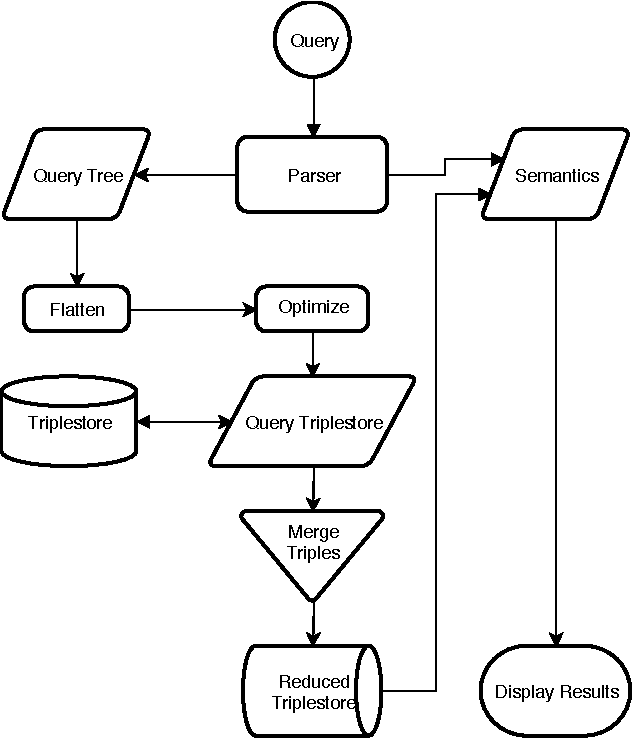
\includegraphics[width=11cm]{images/queryprocess.pdf}
	\caption{Application architecture.}
\end{figure}
%\begin{figure}
%	\vspace{-2.0em}
%	\centering
%	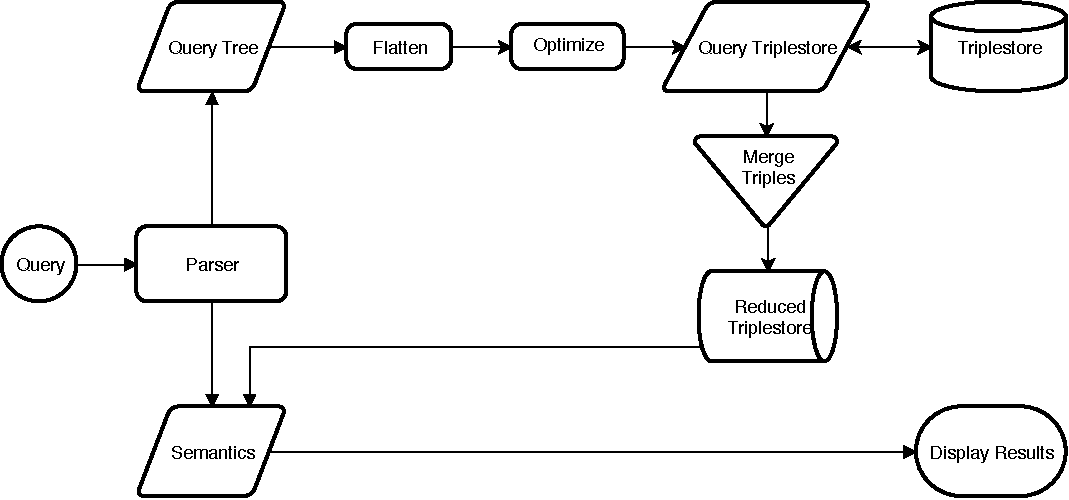
\includegraphics[width=\textwidth]{images/queryprocess2.pdf}
%	\caption{Application architecture.} \label{fig1}
%	\vspace{-2em}
%\end{figure}

\noindent The query begins as a string of text as sent to the semantics, which is then sent directly to the parser, as described in \Cref{webist2019journal:compositionality-syntax}.  This produces two results:

{
\renewcommand\labelenumi{(\theenumi)}
\begin{enumerate}
	\item A function that, given a set of triples, will evaluate the query with respect to that set of triples and return the result
	\item A ``\textit{Memo Tree}'' that roughly follows the syntax tree resulting from the parse of the input string. In addition to providing a unique name to each sub-expression of the parsed input, it is also used to determine which queries need to be evaluated against the remote triplestore.
\end{enumerate}
}

\noindent The function produced in (1) requires a set of triples to produce a result.  While it is possible, given sufficient time and resources, to directly retrieve all triples from the remote triplestore and pass them directly into this function to evaluate the input, in practice it is cost prohibitive to do so.

Instead, we retrieve only {\em relevant triples} \cite{peelar2016accommodating} from the remote triplestore and we create a {\em reduced} triplestore from them which is then passed into (1). The Memo Tree obtained in (2) is traversed to obtain the set of all triplestore queries that are required to evaluate each sub-expression of the parsed input.  These queries correspond to the \texttt{getts} family of functions described in \Cref{webist2019journal:getts}. The results of these queries may \textit{overlap}, i.e. share triples in common with those of other queries in the set. An optimization step is performed to eliminate these redundant queries. Domain specific knowledge could be used to improve this process where appropriate.
Finally, these optimized queries are evaluated against the remote triplestore and the results are merged and stored locally in the reduced triplestore.  These triples are then passed to the function produced in (1), yielding the final result.
This is one area where our NLQI differs from other NLQIs to the Semantic Web -- notice that nowhere do we attempt to directly translate the NL query into SPARQL or any other querying language.  Instead, we rely on simple triple querying primitives which are embedded in the semantics to perform this task for us.

The architecture presented in this section lends itself to a very clean implementation in Haskell, where the semantics themselves can be written as pure functions, with the only impure parts of the NLQI being those that directly deal with querying the triplestore and with presenting these results to the user. We expand on the individual sub-components of the NLQI in the following sections.

\subsection{Triple Retrieval}
\label{webist2019journal:tripleretrieval}

\subsubsection{Remote Triplestore}
\label{webist2019journal:getts}

Our semantics does not directly depend upon any particular query language.
When querying remote triplestores, the NLQI requires only two conceptually simple functions.  The first is:

\examplespacing

\texttt{getts\_triples\_entevprop\_type ev\_data prop\_names ev\_type}

\examplespacing

\noindent This function is used to retrieve triples belonging to the relation \texttt{ev\_type}.  \linebreak \texttt{prop\_names} is a list of columns of the relation to retrieve.  Only the names of the columns of the relation that are actually required are listed here.  Finally, \linebreak \texttt{ev\_data} is the URL used to access the remote triplestore or database.  For example, in the query \texttt{what discovered}, it may be invoked as follows:

%This may point to a SPARQL endpoint, a Triple Pattern Fragment \cite{verborgh2014web} interface, an SQL interface, or an interface to any other type of database where triples may be accessed from.

\examplespacing

\texttt{getts\_triples\_entevprop\_type url ["subject"] "discover\_ev"}

\examplespacing

\noindent This would retrieve the triples of all ``discover'' events that contain a \property{subject} property, including the triples describing the type of those events.  The second function is:

\examplespacing

\texttt{getts\_triples\_members ev\_data set}

\examplespacing

\noindent Here, \texttt{ev\_data} performs the same function as it did previously, and ``\texttt{set}'' indicates the name of a set, for example the moons or the set of things that spin.  This retrieves the triples of all ``membership'' events whose \property{object} property corresponds to that set, including the triples describing the type of those events.

Together, these two primitives can be used to retrieve triples from event-based triplestores, provided the names of the roles to be queried are known.  This would typically be described in a schema, but in simple cases may be feasible to hard-code into a program. To see how these two primitives work in action, consider the following complex query, featuring chained prepositional phrases:

\examplespacing

\texttt{which person discovered a moon in 1877 with a telescope}

\examplespacing

\noindent This would invoke the following queries to the database:

\examplespacing

\texttt{getts\_triples\_entevprop\_type url ["subject", "object",  "year", \linebreak "implement"] "discover\_ev"}

\texttt{getts\_triples\_members url "moon"}

\texttt{getts\_triples\_members url "telescope"}

\texttt{getts\_triples\_members url "person"}

\examplespacing

\noindent These four queries to the remote triplestore, taken together, will retrieve enough information to answer the user's query. Transitive and intransitive verbs are implemented in terms of \texttt{getts\_triples\_entevprop\_type}. Common nouns and adjectives are implemented in terms of \texttt{getts\_triples\_members}.  These conceptually simple functions are easy to implement in SPARQL, SQL, and as Triple Pattern Fragments \cite{verborgh2014web}.  An example implementation is provided in our source code, available on Hackage \cite{xsaiga} for both Triple Pattern Fragments and SPARQL.

After all ``\texttt{getts}'' queries are evaluated, their results are merged together into a local {\em reduced} triplestore.  The idea behind this triplestore is that it contains enough triples to evaluate the correct result, but no more than that.  In other words, the results from passing in the entire triplestore to the semantic function in (1) and the results from passing in the reduced triplestore should be equivalent.

\subsubsection{Reduced Triplestore}

Once the reduced triplestore is passed into the semantics, however, it still needs to be queried by the semantic functions in the denotations.  This is where the boundary of the impure code of the NLQI meets the pure code of the semantics. At this higher level, there are three primitives that are used to query the reduced triplestore:
\begin{itemize}
	\item \texttt{pure\_getts\_triples\_entevprop\_type ev\_data prop\_names ev\_type}

	\item \texttt{pure\_getts\_triples\_entevprop ev\_data prop\_names evs}

	\item \texttt{pure\_getts\_members ev\_data set}
\end{itemize}
These are very similar functions to those described previously, however they are implemented as pure functions in Haskell.  The actual implementation of the reduced triplestore is opaque to the semantics, which rely strictly on these three functions to retrieve triples from the reduced triplestore.  Implementing these as pure functions allows them to be embedded in the semantics, which are implemented as pure functions themselves.  This provides a number of benefits, including allowing the semantics and queries to be lazily evaluated.
\texttt{pure\_getts\_triples\_entevprop\_type} performs a similar role as it did previously. \texttt{pure\_getts\_triples\_entevprop} is a new function that, instead of specifying an event type parameter, specifies a set of events instead.  This is used to implement chained prepositional phrases, where sets of events are honed down in the order that the phrases occur in (from left to right).  Finally, \texttt{pure\_getts\_members} performs a similar function as it did previously, except this time it directly returns an FDBR from the members of the set given to the events in which the set membership is recorded.

%The pure versions of the ``\texttt{getts}'' functions do not need to retain the \textit{ev\_type} property in the set of triples returned, unlike the impure versions.  If this property were lacking from the results of the impure versions, it would be impossible to know which relations that the triples belonged to in the reduced triplestore.

\subsection{Handling Ambiguity in the Query Interface}
\label{webist2019journal:ambiguity}

\subsubsection{Syntactic ambiguity}
As queries may be ambiguous, it's important that users see how their queries were parsed to understand the result given.  Our system displays the parse tree along with the query result to assist with this.  The parse tree is presented in a familiar Haskell syntax to indicate scoping.  As an example, consider the scoping of the simple query ``\texttt{who discovered a moon that orbits mars}'':

\examplespacing

\texttt{who (discovered (a (moon `that` (orbits mars))))}

\examplespacing

\noindent Here, we see that scoping of denotations is shown with parentheses.  Prepositional phrases are enclosed inside square brackets, with commas to delimit chained prepositional phrases:

\examplespacing

\texttt{who discovered a moon in 1877 with a telescope}

\qquad $\Rightarrow$ \texttt{who (discovered (a moon) [in 1877, with (a telescope)])}

\examplespacing

\noindent This mirrors the familiar list syntax that Haskell offers and suggests to the user that the prepositional phrases will be evaluated in the order presented (left to right), allowing users to understand exactly how their query is evaluated by the system. Now, consider the following ambiguous query:

\examplespacing

\texttt{who discovered a moon that orbits in 1877}

\examplespacing

\noindent There are two possible parses of this query, depending on which transitive verb the prepositional phrase ``\texttt{in 1877}'' is applied to:

\examplespacing

\texttt{who (discovered (a (moon `that` (orbits [in 1877]))))} $\Rightarrow \opit{none}$

\texttt{who (discovered (a (moon `that` orbits)) [in 1877])} $\Rightarrow  \opit{hall}$

\examplespacing

\noindent In the first case, the prepositional phrase ``\texttt{in 1877}'' is treated as though it applies to ``\texttt{orbits}''.  However, the result is ``\textit{none}'' because orbit events do not have a concept of time in our database.  If we were to add a \property{year} role to the ``orbit'' relation, then all planets and moons in the solar system would be returned.
In the second case, ``\texttt{in 1877}'' applies to ``\texttt{discovered}'', a relation which has the concept of a time of discovery (the \property{year} role).  As \texttt{hall} is the only person that discovered anything in 1877, only they are included in the result.

Our system permits highly ambiguous input, providing a result for each possible parse of that input.  However, it may be the case that a user has a clear understanding of how they want their query to be parsed and would gain no benefit from seeing other possible parses of their query.  Fortunately, this use case is easily accommodated with a simple extension to our NLQI: allowing the scoping syntax as presented above directly in the query interface itself.  For example, a user could directly query ``\texttt{what (discovered (a (moon `that` orbits)) [in 1877])}'', which would exclude the other parse as mentioned in the example above.  In fact, the query need not even be fully explicitly scoped to benefit from this.  A partial scoping such as ``\texttt{what discovered (a moon that orbits) in 1877}'' would be sufficient to exclude the other undesirable parses from the result.  We intend to implement this functionality in our NLQI in the very near future.

It may also be worthwhile to implement a simple dialogue-based approach to disambiguation, where the system could simply provide the possible parses to the user and allow them to choose which one they intended.  This approach may be beneficial when using speech to interact with the system, as providing scoping with the above method directly with speech would be very inconvenient.  An example dialogue could be:

\examplespacing

\noindent \textbf{User:}

\texttt{what discovered a moon that orbits mars in 1877 with a telescope}

\noindent \textbf{Interface:}

\texttt{There are three possible ways I can interpret this query.}

\texttt{Which one do you mean?}

\texttt{1) what (discovered (a (moon `that` (orbits mars [in 1877,\linebreak with (a telescope)]))))}

\texttt{2) what (discovered (a (moon `that` (orbits mars))) [in 1877,\linebreak with (a telescope)])}

\texttt{3) what (discovered (a (moon `that` (orbits mars [in 1877])))}

\noindent \texttt{[with (a telescope)])}

\noindent \textbf{User:}

\texttt{2}

\noindent \textbf{Interface:}

\texttt{OK -- the result of the second interpretation is ``hall''}

\examplespacing

\noindent If the modality of the interface is by voice, reading the scoping directly as presented above may be inconvenient to users.  Fortunately, it is possible to verbally state the scoping in an intuitive way:

\examplespacing

\noindent \textbf{User:}

\texttt{what discovered a moon that orbits mars in 1877 with a telescope}

\noindent \textbf{Interface:}

\texttt{I can interpret this three different ways. In the first interpretation, the prepositions ``in 1877'' and ``with a telescope'' apply to the verb ``orbit''.  Is that what you meant?}

\noindent \textbf{User:}

\texttt{no}

\noindent \textbf{Interface:}

\texttt{In the second interpretation, the prepositions ``in 1877'' and \linebreak ``with a telescope'' apply to the verb ``discovered''.
	Is that	\linebreak what you meant?}

\noindent \textbf{User:}

\texttt{yes, that's what i meant}

\noindent \textbf{Interface:}

\texttt{OK -- the result of that interpretation is ``hall''}

\examplespacing

\abbreviation{NLP}{Natural Language Processing}
\noindent Given the different nature of the user's responses compared to the queries themselves, they may be subject to a different grammar or may be handled by a different system entirely that permits more free-form responses to be given. This could be a good opportunity to integrate Machine Learning-based Natural Language Processing (NLP) approaches in the NLQI in the future, as they are ideally suited to use cases involving loosely structured input.

\subsubsection{Semantic Ambiguity}

Semantic ambiguity may also be accommodated by permitting multiple definitions of the same terminal in the grammar, augmenting it with a human readable description of what the terminal means.  Each definition would be evaluated as though it were a different parse of the query, although each parse would have the same syntax tree.  To avoid confusion, the human readable definition of the word could be printed below the tree.

\subsection{Semantic Implementation}

The semantics themselves are completely unaware of the structure of the underlying triplestore and the methods and query languages used to retrieve triples from it.
Recall from \Cref{webist2019journal:architecture} that the result of a parse of user input produces two items: a pure function that, given a triplestore as input will produce the result of a query and a tree that represents the query itself, including the types of queries that are required from a remote triplestore.

\subsubsection{Applying Multiple Semantics in Parallel}

The Biapplicative Bifunctor in Haskell, which is inspired from its counterpart in category theory, can serve as a generalization of function application.  One possible use for it is to apply pairs of values to pairs of functions.  Briefly, given two arbitrary functions $f$ and $g$
and two values $a$ and $b$ we can use the biapplicative operator \texttt{<<*>>} to apply $a$ and $b$ both functions in parallel: $(f, g)$ \texttt{<<*>>} $(a, b) = (f\ a, g\ b)$.  The functions themselves need not be related.
First, we introduce an operator, \texttt{>|<}, that allows us to bridge together two semantics such that they can be applied using \texttt{<<*>>}:
\begin{equation*}
	a\ \texttt{>|<}\ b = (a, b)
\end{equation*}
This allows these two independent functions to be applied in parallel while parsing the input string using the exact same grammar and no code duplication, provided the \texttt{<<*>>} is used in place of function application.  For example, ``\texttt{a moon spins}'' is evaluated as though it were written as ``\texttt{a <<*>> moon <<*>> spins}'' under this approach.  Our NLQI uses this to construct the Memo Tree in parallel while applying the denotations of the words in the query.  Consider the following example, where GIntersect and GMembers are constructors of the Memo Tree:

\begin{code}
    a' = a >|< GIntersect
    moon' = moon >|< GMembers "moon"
    spins' = spins >|< GMembers "spins"
\end{code}
Therefore,
\begin{code}
    a' <<*>> moon' <<*>> spins'
    => (a moon spins, GIntersect (GMembers "moon") (GMembers "spin"))
\end{code}
However, this is somewhat inconvenient and unfamiliar syntax to work with. Fortunately, it is trivial to define a set of ``wrapper'' functions to restore the original function application syntax:
\begin{equation*}
	\begin{split}
		%	&\opit{wrap}_1\ (f, g)\ (a_1, b_1) =\ (f\ a_1,\ g\ b_1) \\
		%	&\opit{wrap}_2\ (f, g)\ (a_1, b_1)\ (a_2,b_2) = (f\ a_1\ a_2,\ g\ b_1\ b_2) \\
		%	&\ldots \\
		&\opit{wrap}_N\ (f, g)\ (a_1, b_1)\ (a_2,b_2)\ \ldots\ (a_N, b_N) = (f\ a_1\ a_2 \ldots a_N,\ g\ b_1\ b_2 \ldots b_N)
	\end{split}
\end{equation*}
Here, the function $\opit{wrap}_N$ takes a pair of functions $(f, g)$ with arity $N$ and then $N$ pairs of arguments to be applied in order to $f$ and $g$ respectively.  This allows ``\texttt{a' <<*>> moon' <<*>> spins'}'' above to be written as ``$\mathtt{a'\ moon\ spins}$'', where $\mathtt{a''} = \opit{wrap}_2\ \mathtt{a'}$.
%While it is possible in languages with sufficient meta-programming facilities to define $\opit{wrap}_N$ generically and deduce $N$ from its context, i.e. from the pair of functions it is applied to, for our purposes it is not necessary to do so.In the semantics as described, each function needs only two arguments at most, and the types are \_.
%Note that this approach generalizes to $N$ semantic functions by using $N$-applicative $N$-functors and modifying $\opit{wrap}_N$ accordingly.
Therefore, we can retain the familiar function application syntax in the semantics while taking advantage of parallel function application. By itself, this is a convenience, but let us revisit the Memo Tree once more. It has two uses. The first is as stated previously, in determining which queries need to be performed against the remote triplestore. The second is that this allows us to assign a unique identifier to each sub-expression of the parsed input.

\subsubsection{Memoized Compositional Semantics}
\label{webist2019journal:memoization}

Consider the query ``\texttt{what is orbited by a thing that was discovered by a person that discovered phobos}'', containing three nested transitive verbs.
One possible parse of this query yields:
\begin{center}
	\texttt{what (is orbited [by (a (thing `that` (was discovered [by (a (person `that` (discovered phobos)))])))])}
\end{center}
A query's sub-expressions may be evaluated multiple times during the prepositional filtering of a transitive verb (i.e one evaluation for each row of the FDBR denoted in that transitive verb).  This has a compounding effect when transitive verbs are nested as sub-expressions in prepositional phrases of other transitive verbs. In general, if there are $m$ nested transitive verbs in a query, each having an FDBR with $n$ rows. then the complexity for evaluation is $O(n^m)$.

As it turns out, we can use the Memo Tree to memoize the results of the sub-expressions of a query, drastically reducing the number of re-evaluations performed.  The memoization occurs in a more sophisticated version of the $\opit{wrap}_N$ functions described previously, which use the unique identifier provided by the Memo Tree to memoize the results of the semantic functions as they are evaluated. This is completely transparent to the user, and the familiar function application syntax used in all previous examples still remains. This reduces the complexity to $O(mn)$, where $m$ is the number of nested transitive verbs, each having an FDBR with $n$ rows. All sub-expressions in the query are memoized, including the final result of the query expression itself.

%In this memoization scheme, the results of the sub-expressions as listed previously are retrieved without needing to be re-evaluated.
%TODO: As an example, in the query above, the first time ``\texttt{thing `that` (was discovered [by (a (person `that` (discovered phobos)))])}'' is evaluated during prepositional filtering of \texttt{orbited}, it is memoized, and later references to this sub-expression retrieve the memoized value.
%As an example where memoization would improve evaluation time, consider the query  ``\texttt{what is orbited by a thing that spins}''.
%One possible parse of this query yields ``\texttt{what (is orbited [by (a (thing `that` spins))])}''.
%Here, ``\texttt{thing `that` spins}'' needs to be evaluated for each row in the FDBR of ``orbited'', where the events of each row $r$ are gathered into a new FDBR $f$ and the events of $r$ are replaced with $\meaningof{a}\ \meaningof{thing\ that\ spins}\ f$.  However, \texttt{thing that spins} will evaluate to the same FDBR for each row, and it can be cached -- only the second argument to $\meaningof{a}$ is changing for each row.  However, ``\texttt{thing `that` spins}'' is relatively simple to evaluate.
%
%Now consider the following query, which contains many nested subexpressions including transitive verbs:
%\begin{center}
%	\texttt{what is orbited by a thing that was discovered by a person that discovered phobos}
%\end{center}
%One possible parse of this query yields:
%\begin{center}
%\texttt{what (is orbited [by (a (thing `that` (was discovered [by (a (person `that` (discovered phobos)))])))])}
%\end{center}
%Again, each row of the FDBR denoted by ``\texttt{orbited}'', needs to evaluate ``\texttt{by (a (thing `that` (was discovered [by (a (person `that` \linebreak (discovered phobos)))])))}'', and each row of the FDBR denoted by ``\texttt{discovered}'' needs to evaluate ``\texttt{by (a (person `that` (discovered phobos)))}''.
%The results of these function applications remain the same during each evaluation, with the only difference being the FDBR obtained from the set of events in the row of the FDBR they are being \textit{intersect}ed with during prepositional filtering.  If there are $m$ nested transitive verbs in a query, each having an FDBR with $n$ rows, then the complexity for evaluation is $O(n^m)$.
%However, using the memoization scheme described previously, the situation improves drastically.  The results of the subqueries as listed previously are retrieved without needing to be re-computed during intersection with the sets of events in each row of the FDBRs.  This reduces the complexity to $O(mn)$ where $m$ is the number of nested transitive verbs, each having an FDBR with $n$ rows.
The State monad in Haskell is used to thread the memoized state throughout the execution of the semantics.  This mirrors the memoization technique used in the parser itself to provide efficient parsing using combinators \cite{frosthafiz2008}.
We believe this two-pronged approach to triplestore retrieval and memoization is novel and has not been used in any other Compositional Semantics-based systems.  We intend to expand more on our approach in a future publication, as we believe it to be useful for creating modular and efficient compositional NLQIs that can scale to the needs of the Semantic Web.  For example, this approach could be used for developing NLQIs for low-power embedded devices that are suitable for IoT applications.

\section{Related Work}
\label{webist2019journal:relatedwork}

Orakel \cite{cimiano2007orakel} is a portable NLQI which uses a Montague-like grammar and a lambda calculus semantics. Our approach is similar in this respect. Queries are translated to an expression of first order logic enriched with predicates for query and numerical operators. These
expressions are translated to SPARQL or F-Logic. Orakel supports negation, limited quantification, and simple prepositional phrases.

YAGO2 \cite{hoffart2013yago2} is a semantic knowledge base containing reified triples extracted from Wikipedia, WordNet and GeoNames, representing nearly 0.5 billion facts. Reification is achieved by tagging each triple with an identifier. However, this is hidden from the user who views the knowledge base as a set of ``SPOTL'' quintuples, where T is for time and L for location. The SPOTLX query language is used to access YAGO2. SPOTLX can handle queries with prepositional aspects involving time and location. However, no mention is made of chained complex PPs.

Alexandria \cite{wendt2012linguistic} is an event-based triplestore, with 160 million triples (representing 13 million n-ary relationships), derived from FreeBase. Alexandria uses a neo-Davidsonian \cite{parsons1990events} event-based semantics. In Alexandria, queries are parsed to a syntactic dependency graph, mapped to a semantic description, and translated to SPARQL queries containing named graphs. Queries with simple PPs are accommodated. However, no mention is made of negation, nested quantification, or chained complex PPs.

The systems referred to above have made substantial progress in handling ambiguity and matching NL query words to URIs. However, they appear to have hit a roadblock with respect to natural-language coverage. Most can handle simple PPs such as in ``\texttt{who was born in 1918}'' but none can handle chained complex PPs, containing quantifiers, such as ``\texttt{in us\_naval\_observatory in 1877 or 1860}''.

Blackburn and Bos \cite{blackburn2005representation} implemented lambda calculus with respect to natural language, in
Prolog, and Van Eijck and Unger \cite{van2010computational} have extensively and clearly discussed such implementation in
Haskell. Implementation of the lambda calculus for open-domain question answering has been
investigated by \cite{ahn2005question}.
The SQUALL query language \cite{ferre:squall,ferre2013squall} is a controlled natural language
(CNL) for querying and updating triplestores represented as RDF graphs. SQUALL can return
answers directly from remote triplestores, as we do, using simple SPARQL-endpoint triple
retrieval commands. It can also be translated to SPARQL queries which can be processed by
SPARQL endpoints for faster computation of answers. SQUALL can handle
quantification, aggregation, some forms of negation, and simple unchained prepositional phrases containing the word ``\texttt{at}'' and ``\texttt{in}''.  It can also handle superlative phrases as long as they are not nested under a prepositional phrase.  Notably, the scope of prepositional phrases in SQUALL are the entire sentence they reside in.
It is also written in a functional language. However, some queries in SQUALL require the use of variables and low-level relational algebraic operators (see for example, the queries on page 118
of \cite{ferre2013squall}).

%TODO: is this plagiarism since it was in the ICSC paper?
%TODO: Richard needs to look over the SQUALL section

\section{Future Work}
\label{webist2019journal:futurework}

\subsubsection{Negation}
Our system currently relies on the Open World Assumption, where the absence of evidence cannot be treated as having evidence of absence.  As a consequence of this, the system currently is unable to handle negation, and does not have a denotation for the words ``\texttt{no}'' and ``\texttt{not}''.

However, there is a clear need for handling negation in our semantics where the Closed World Assumption holds. For example, it should be possible to answer queries such as ``\texttt{who did not discover a moon}'' or ``\texttt{what discovered no moon}''.  Work has been done on event-based semantics that can handle negation \cite{champollion2015interaction}.  We believe it should be possible to accommodate negation in our semantics as well using a similar approach, and in turn provide a denotation for ``\texttt{the least}'' as well, as noted in \Cref{webist2019journal:superlatives}.

\subsubsection{DBPedia}

%NOTE: our system might be able to directly use YAGO3
With the addition of memoization in our semantics, we feel our approach is now scalable enough to work directly with DBPedia.  We intend to expand on how our semantics can handle large triplestores such as DBPedia in a future publication.  In particular, an interface to DBPedia will allow our approach to be directly evaluated with existing systems in use, such as YAGO \cite{hoffart2013yago2}.

\subsubsection{Hardware Acceleration}
Consider that the reduced triplestore described in \Cref{webist2019journal:tripleretrieval} is stored locally in the query interface and is queried with the pure ``\texttt{getts}'' functions.  These could make good candidates for offloading to FPGA fabric or a GPU for hardware acceleration.
Work has been done in developing on FPGAs using Haskell \cite{baaij2009clambdaash}.
This could allow for both low latency and low power consumption in embedded consumer devices, such as those that operate on the Internet of Things.

\subsubsection{Non-Event-Based Triplestores}
We also believe it should be possible to handle non-event based triplestores as well using our approach using a translation layer.  It may be possible to use ontological information to provide an event-based view to many kinds of non-event based data.  Machine Learning approaches could provide a way forward in the absence of or lacking sufficient ontological information about a triplestore.

\section{Conclusions}
\label{webist2019journal:conclusions}

This work comes at an appropriate time when massive triplestores, such as DBpedia \cite{dbpedia} are being created containing billions of verified facts. We are currently looking at how such facts can be converted to event-based triples which can be queried by our interface.
We are confident that, after we accommodate negation, our compositional semantics is appropriate for answering most queries that are likely to be asked of data stores containing domain-specific knowledge. We have shown how the FDBR data structure presented in this paper can be used to handle many kinds of complex language features, including chained prepositional phrases and superlatives. The way quantification is handled within the semantics is consistent with other work in this area, as discussed in \Cref{webist2019journal:quant}. Our approach is extensible enough that it can accommodate queries to both relational and non-relational types of database, including Semantic Web triplestores. Our approach is also suitable for use on low power devices, which may be useful for applications on the Internet of Things (IoT).

We have shown how our system is tolerant of highly ambiguous user input and we discussed possible ways to present this in \Cref{webist2019journal:ambiguity}.  In particular, we discussed how both semantic and syntactic ambiguity could be handled.
We also presented a novel approach to memoizing compositional semantics using unique identifiers attached to sub-expressions in a query, substantially improving the time complexity of evaluation. We also showed how those unique identifiers are also useful to determine the set of queries that need to be made to the remote database.

Our next goal is to provide an NLQI to DBPedia using our approach with the techniques described here, and then evaluate the effectiveness of our system relative to other NLQIs using established benchmarks, such as QALD \cite{qald9}.

%In the future, we plan to scale up the capability of our NLQI further to access massive data stores such as DBpedia. To achieve this goal, we plan to accelerate the FDBR generation process using specialized acceleration hardware, such as FPGAs and GPUs.

%We are also able to accommodate many concurrent users with a recent extension that allows the interface to be executed in a web browser which only uses the remote server to retrieve triples from the triplestore.

%We are confident that, after we accommodate negation, our compositional semantics is appropriate for most queries that are likely to be asked of data stores containing everyday knowledge.
%The FDBR data structure presented in this paper can be used to handle many kinds of complex language features, including chained prepositional phrases and superlatives.  The way quantification is handled within the semantics is consistent with other work in this area, as discussed in \Cref{sec:quant}.
%The approach chosen is flexible enough that it can accommodate queries to both relational and non-relational types of databases, including Semantic Web triplestores.  It is also suitable for use on low power devices, which may be useful for applications on the Internet of Things (IoT).
%
%In the future, we plan to scale up the capability of our NLQI further to access massive data stores such as DBpedia.  To achieve this goal, we plan to accelerate the FDBR generation process using specialized acceleration hardware, such as FPGAs and GPUs.

%\pagebreak
%TODO: these need to be numbered from 1 each time
\printbibliography[heading=subbibintoc]
\end{refsection}

\end{document}
